%!TEX root = ../thesis.tex

\section{ROS 2}
ROS 2(Robot Operating System versition 2)は, オープンソースのロボットソフトウェアフレームワークであり,
ロボットアプリケーションの開発や実行をサポートするミドルウェアである.
異なるバージョンが存在しているが, 本研究ではROS 2 foxyを主に使用している.

\subsection{RViz2}
RViz2(ROS VIsualization2)はROS 2で提供される三次元ビジュアライゼーションツールであり, 
数値で表されるロボットの座標や各センサのデータを視覚的に表すことができる.

\begin{figure}[H]
  \centering
 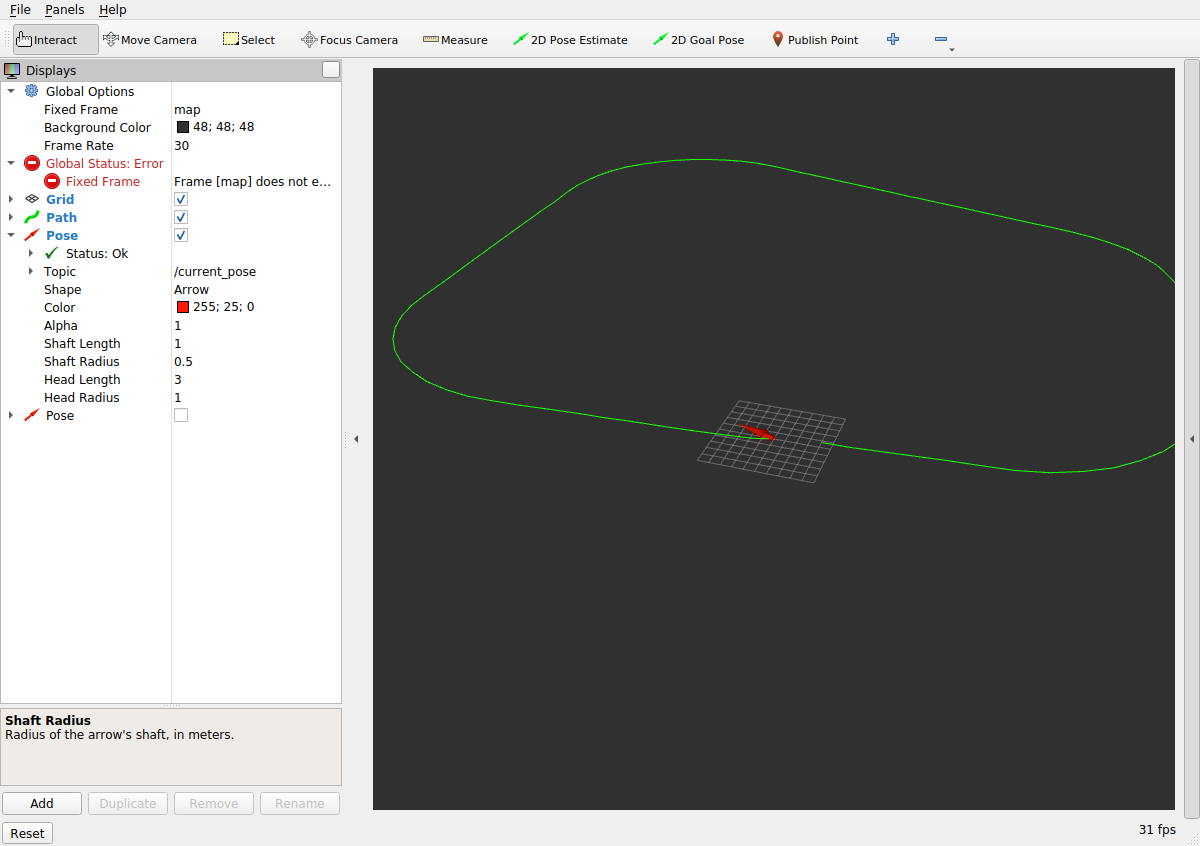
\includegraphics[keepaspectratio, scale=0.4]
     {images/rviz.png}
 \caption{RViz2 view}
 \label{fig:purepursuit}
\end{figure}

\section{GNSS}
GNSS(Global Navigation Satelite System)は, 
人工衛星を利用して地上の現在位置を計測するためのシステムであり, 
アメリカのGPS, ロシアのGLONASS, ヨーロッパのGalileo, 日本のQGSSなどを総称した衛生測位システムを指す.

計測する値は衛生と受信機(アンテナ)間の距離であり, 衛生位置を既知として受信機の三次元座標と受信機時計の誤差を未知数として最低4つの観測値から座標計算される.
測定された距離にはさまざまな誤差要因が含まれる.

\subsection{UTM座標系}
UTM(Universal Transverse Mercator)座標系とは, 全世界を経度6度ごとのゾーンに分けて東回りに番号を付けて規格化したものである.
世界的にも大・中縮尺の図法として採用され, 日本では国土地理院の地形図や地勢図で採用されている.

\begin{figure}[H]
  \centering
 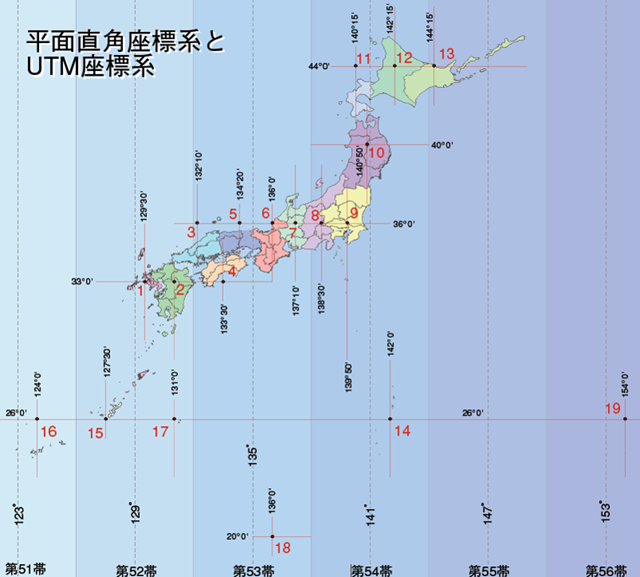
\includegraphics[keepaspectratio, scale=0.7]
      {images/UTMCoordinateSystem.png}
 \caption{UTM Coordinate System(source)}
 \label{fig:UTM}
\end{figure}

% AIFormulaの会場となるAIモビリティパークは茨城県常総市にあるため, 54帯のUTM座標系を使用する.

\subsection{ECEF座標系}
ECEF(Earth-Centered, Earth-Fixed)座標系とは, 地理的・直交的な座標系であり, 地球の自転と同期して常時回転している座標系である.

\subsection{測地座標系}
測地座標系とは, 地球上の位置を緯度, 経度, および回転楕円体からの高さで表す座標系である.

\subsection{マルチパス}
マルチパスとは, 電波がまっすぐに届くだけでなくビルなどの高層建造物に反射して複数のルートを通って伝播することである.
反射した電波は到達するまでにわずかな遅れを生じ, 遅れの時間の分だけ距離が遠いと計測されてしまうため, 正確な測位を乱す要因の一つとなっている.

\begin{figure}[H]
  \centering
 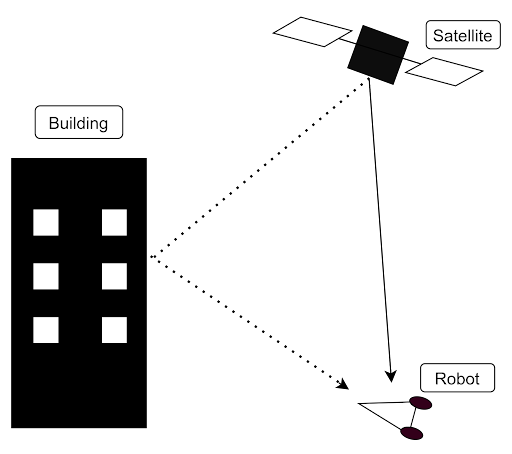
\includegraphics[keepaspectratio, scale=0.4]
      {images/multipath.png}
 \caption{Multipath}
 \label{fig:multipath}
\end{figure}

\section{IMU}
IMU(Inertial Measurement Unit)は, 
3次元の慣性運動を検出する装置である. 
加速度センサーにより並進運動を検出し, 
ジャイロセンサーにより回転運動を検出することができる.

\newpage